\documentclass{bioinfo}

\usepackage{relsize} % for Cpp
\usepackage{xspace} % for Cpp
\usepackage{subfigure}

\usepackage{natbib}

\newcommand{\odgi}{ODGI}
\newcommand{\vg}{VG}

\newcommand{\FIXME}{\textbf{!!FIXME!!}}
\newcommand{\cmd}[1]{{\scriptsize\textrm{#1}}}
\newcommand{\cmdbf}[1]{{\textbf{#1}}}
\newcommand{\topic}[1]{{\cmdbf{#1}}:}
\newcommand{\Rplus}{\protect\hspace{-.1em}\protect\raisebox{.35ex}{\smaller{\smaller\textbf{+}}}}
\newcommand{\pp}{\Rplus\Rplus}
\newcommand{\Cpp}{\mbox{C\Rplus\Rplus}\xspace}


\copyrightyear{2021} \pubyear{2021}

\access{Advance Access Publication Date: Day Month Year}
\appnotes{Application Note}

\begin{document}
    \firstpage{1}

    \subtitle{Pangenome analysis}

    \title[ODGI: scalable tools for pangenome graphs]{ODGI: scalable tools for pangenome graphs}
    \author[Guarracino, Heumos \textit{et~al}.]{
        Andrea Guarracino\,$^{\text{\sfb 1,}\dagger,*}$,
        Simon Heumos\,$^{\text{\sfb 2,}\dagger}$,
    % XXXXX,
        Pjotr~Prins\,$^{\text{\sfb 3}}$ and
        Erik~Garrison\,$^{\text{\sfb 3,}*}$
    }
    \address{$^{\text{\sf 1}}$Biology, University of Tor Vergata, Rome, 00133, Italy \\
        $^{\text{\sf 2}}$QBiC, University of Tübingen, Tübingen, XXXXXXXXXX, Germany \\
        $^{\text{\sf 3}}$Genetics Genomics \& Informatics, UTHSC, Memphis, TN, USA
    }

    \corresp{$^\ast$To whom correspondence should be addressed.}
    \corresp{$^\dagger$The authors wish it to be known that the first two authors should be regarded as joint First Authors.}

    \history{Received on XXXXX; revised on XXXXX; accepted on XXXXX}

    \editor{Associate Editor: XXXXXXX}

    \abstract{ \textbf{Motivation:} Pangenomes address the
      shortcomings of mainline genomics workflows, in particular
      concerning reference genome bias and identification of complex
      structural variants.
        %
        \\ \textbf{Results:} Here we present \odgi\, a novel range of
        scalable tools that makes use of an efficient in-memory
        representation of DNA graphs. \odgi\ can handle hundreds of
        large genomes at the same time while maintaining fast
        execution runtime and low memory overheads.  \odgi\ includes
        tools for detecting complex regions, extracting \textit{loci},
        exploratory analysis, sorting, removing artifacts, and graph
        manipulation and visualisation.
        %
        \\
        \textbf{Availability:} \odgi\ is software written in the \Cpp\ programming language and
        published under the permissive MIT license. Source code and user manual can be downloaded from
        \href{https://github.com/pangenome/odgi}{https://github.com/pangenome/odgi}.\\
        %
        \textbf{Contact:}
        % \href{andreaguarracino@outlook.com}{andreaguarracino@outlook.com},
        egarris5@uthcs.edu\\
        \textbf{Supplementary information:} Supplementary data are available at \textit{Bioinformatics} online. \FIXME}

    \maketitle

    

\begin{figure*}[ht]
  \vspace{-10pt}
   \begin{minipage}[b]{\textwidth}
  % \begin{center}

    \subfigure[aligned MHC pangenome]{
      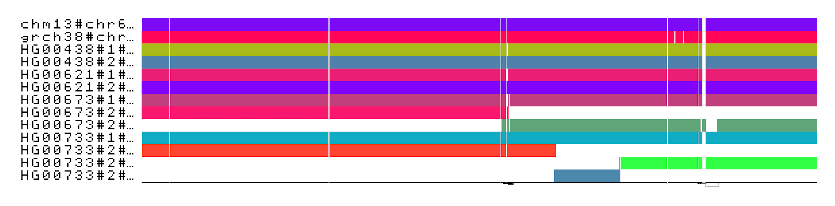
\includegraphics[width=.48\textwidth]{fig/mhc-align.eps}
      \label{subfig1}
    }
    \vspace{-11pt}
    % \newline
    \subfigure[consensus MHC pangenome]{
      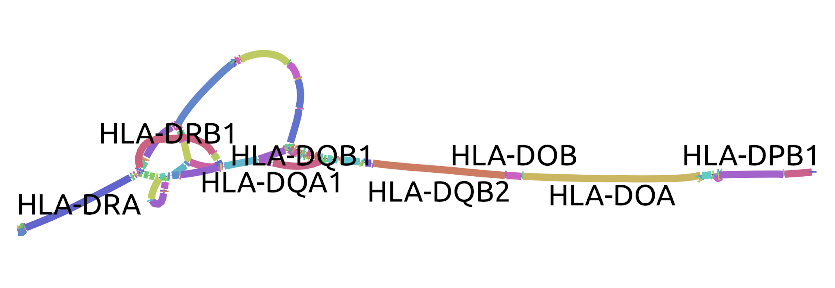
\includegraphics[width=.48\textwidth]{fig/mhc-pangenome.eps}
      \label{subfig2}
    }
            \caption{(b) Visualizing the Major Histocompatibility Complex
                (MHC) \textit{locus} pangenome. A) \cmd{odgi viz} 1D visualization
                of 8 haploid, phased human genome assemblies plus the chm13
                and GRCh38 reference genomes. Graph nodes’ are arranged
                from left to right. The colored bars represent the
                linearized renderings of the embedded paths versus the nodes
                in a binary matrix. The black lines under the paths are the
                links, which represent the graph topology. B)
                Bandage~\citep{26099265} representation of the graph
                topology of a consensus MHC pangenome graph representing
                only variations bigger than 100 bps. Gene labels were
                applied exploiting \cmd{odgi position} to liftover gene
                coordinates from the full graph into the consensus graph.  }

  % \end{center}
  \end{minipage}
\end{figure*}


    \section{Introduction}

    Thanks to advances in sequencing technologies, new genome
    assemblies are produced at a high rate, including the human
    pangenome reference consortium (HPRC) and telomere-to-telemere
    efforts, e.g.~\citep{Miga:2020}.  A pangenome models the full set
    of genomic elements in a given species or clade. Pangenomics
    therefore contrasts with reference genome based approaches which
    relate sequences to a particular consensus model of the
    genome~\citep{Eizenga:2020}. A pangenome can elegantly be
    represented by a graph data structure incorporating sequences as
    nodes and their connections as edges. These nodes are shared for
    homologs, paralogs and orthologs.  A `bidirected' graph represents
    both strands of DNA and so-called paths represent contigs that run
    through the nodes. A path can represent an individual chromosome
    or part thereof. Such a graph-based approach is particularly
    relevant for highly repetitive regions. Segmental duplications,
    and acrocentric chromosomes lead to graphs which present very high
    node depths which greatly increases processing complexity.

    A major challenge is writing software that can deal with the sheer
    size of these graphs representing hundreds, and soon thousands, of
    human genomes. The \vg\ toolkit pioneered graph
    processing~\citep{vgtools,Eizenga:2020b}, but was not designed for
    large data (see Table~\ref{tab:02}). With \odgi\ we
    wrote a new toolset and API in \Cpp\ named Optimized Dynamic
    Genome/Graph Implementation (ODGI). \odgi\ implements a efficient
    graph structure in RAM that can be dynamically updated using
    multiple CPUs.

    Note that \odgi\ is focused on `first-order' graph
    operations.  Other tools are required to construct graphs from raw
    sequences, map reads, or call variants.  \odgi\ provides
    operations on an existing graph, such as subset, subdivide, break,
    combine, normalize and order its components, nodes, and
    paths. Most of the tools are designed to be applied together,
    piping the output of one tool into the next.

    \vspace{-0.1in}

    \section{Results}

    \odgi\ is designed to build and modify paths in parallel. It
    applies concepts first introduced in the dynamic version of the
    graph extension of the positional Burrows-Wheeler
    transform~\citep{Siren:2020}. For implementation details see the
    \odgi\ online documentation. \odgi\ includes the following tools:

    \indent \topic{odgi build, view \& validate} pangenome graphs can be
    stored in the textual Graphical Fragment Assembly
    (GFAv1) format\citep{GFA}; \cmd{odgi build} and \cmd{odgi view}
    convert graphs from GFA to the \odgi\ format and \textit{vice versa}.
    \cmd{odgi validate} ascertains the graph data is correct, such as
    validating that paths respect the graph's topology.

    \topic{odgi viz, sort, draw \& layout} pangenome visualisation
    provides convenient insight into genomic variation. \cmd{odgi viz}
    generates a linearized representation of the pangenome and is
    capable of handling full length human chromosomes
    (Fig.~\ref{fig:1}a). \cmd{odgi sort} reorganises node order and
    simplifies the graph by applying several algorithms, including the
    novel `Path-Guided Stochastic Gradient Descent' algorithm.
    \cmd{odgi layout} generates a file with the X-Y coordinates for
    all nodes and \cmd{odgi draw} draws a layout of the graph
    (Fig.~\ref{fig:1}b).

    \topic{odgi stats, bin, depth \& degree} pangenome numerical
    counts provide insight into genome complexity in other
    ways. E.g., \cmd{odgi stats} returns the number of nodes,
    edges, paths, and graph length. \cmd{odgi bin} summarises path
    information into bins of a specified size, thereby enabling a
    summarised view of large genomes. \cmd{odgi depth} and
    \cmd{odgi degree} return the node depth and degree as defined by
    user provided criteria. These methods allow detection of complex
    genomic regions.

    \topic{odgi break, groom, chop \& unchop} pangenome graphs can be
    reorganised.  \cmd{odgi break} removes circular structures in the
    graph, thereby reducing complexity. \cmd{odgi groom} removes
    spurious inverted links by aligning the graph from the orientation
    that is supported by most paths. \cmd{odgi chop} divides long
    nodes into shorter ones at a maximum requested size, thereby
    simplifying downstream analysis.  \cmd{odgi unchop} joins nodes
    and embedded sequences that do not change the graph topology,
    thereby obtaining a more compact representation of the graph.

    \topic{odgi explode, squeeze \& extract} pangenome are constructed
    as a large graph. \cmd{odgi explode} separates units, such as
    chromosomes, into different files.  \cmd{odgi squeeze} merges
    multiple graphs into the same file whilst preventing node ID
    collisions. \cmd{odgi extract} extracts regions of the graph as
    defined by certain criteria, allowing downstream processing of
    smaller subgraphs.

    \topic{odgi position} pangenome graphs are flexible when it comes
    to coordinate systems. \cmd{odgi position} can use the coordinate
    system from a contained reference genome --- a dynamic liftover
    --- to display coordiates and other localised features, as is shown in
    Fig.~\ref{fig:1b}.


    \section{Discussion}

    Pangenome graphs stand to become a ubiquitous tool in
    genomics\citep{Eizenga:2020}.  With \odgi\ we implemented a
    state-of-the-art tool suite, that can transform, analyse and
    visualise pangenome graphs at scale.  \odgi\ also exposes an API
    that is used by other tools for pangenome graph building and
    normalization. Future work will add support for RNA and protein
    sequences and expand on metadata capabilities of large pangenome
    graphs.

    %TODO to repeat on a bigger machine to avoid vg crashing
    \begin{table}[th]
      \processtable{\small
        Example of performance improvement between
        \cmd{odgi} and \cmd{vg}~\citep{vgtools} equivalent commands with output file
        sizes. The centromere region was extracted from CHR 6 of the
        HPRC year one assembly, i.e., 88~haploid, phased
        human genome assemblies from 44~individuals plus the chm13
        cell line and GRCh38 reference genomes stored in 4.3GB~GFA
        format\citep{GFA}.
        %
        First GFS was converted from GFA to \odgi\ and \vg\
        formats, respectively.  \odgi's path implementation can
        process paths in parallel, outperforming \vg. For the
        same reason \cmd{odgi extract} is $20\times$ faster than
        \cmd{vg chunk} extracting a portion from the full
        graph. \FIXME: vg never finished.
        %
        All timings were performed on a server class machine
        on SSD MODEL with X GB of RAM and 48 CPU cores (Y x 12 core
        AMD Opteron) Processor MODEL @ 3.3 GHz with 8MB L2
        Cache.\FIXME
        % \vspace{0.5in}
        \label{tab:02}}
                   {
                     % \resizebox{.8\textwidth}{!}{
            \begin{tabular*}{.5\textwidth}{@{}lllll@{}}
                \toprule Operation & Tool & Runtime (mm:ss) & Memory (GB) & Output size (GB)    \\
                \midrule
                Format conversion                           &       &       &                   \\
                                    & \cmd{odgi build}      & 1:35  & 10.39 & 5.4               \\
                                    & \cmd{vg convert}      & 8:14  & 28.43 & 6.1               \\
                Subgraph extraction                         &       &       &                   \\
                                    & \cmd{odgi extract}    & 1:15  & 9.43  & 2.7               \\
                                    & \cmd{vg chunk}        & 21:09 & 59.33 & 1.7               \\
                \botrule
            \end{tabular*}} %}

    \end{table}


%\begin{figure}[!tpb]%figure2
%%\centerline{\includegraphics{fig02.eps}}
%\caption{Caption, caption.}\label{fig:02}
%\end{figure}

%%%%%%%%%%%%%%%%%%%%%%%%%%%%%%%%%%%%%%%%%%%%%%%%%%%%%%%%%%%%%%%%%%%%%%%%%%%%%%%%%%%%%
%
%     please remove the " % " symbol from \centerline{\includegraphics{fig01.eps}}
%     as it may ignore the figures.
%
%%%%%%%%%%%%%%%%%%%%%%%%%%%%%%%%%%%%%%%%%%%%%%%%%%%%%%%%%%%%%%%%%%%%%%%%%%%%%%%%%%%%%%

    % \vspace*{+12pt}
    % \textit{Financial Support}: none declared.

    \textit{Conflict of Interest}: none declared.
    % \vspace*{+12pt}

    % \section*{Data availability}

    % Data used to build Human pangenome graphs is available at \href{https://github.com/human-pangenomics/HPP_Year1_Data_Freeze_v1.0}{https://github.com/human-pangenomics/HPP\_Year1\_Data\_Freeze\_v1.0}.

    % \section*{Acknowledgements}
    %ToDo
    % XXXXXXX XXXXXXXX XXXXXXXX XXXXXXXX XXXXXXXX XXXXXXXX XXXXXXXX XXXXXXXX XXXXXXXX.


    % \section*{Funding}
    %ToDo
    % This work has been supported by the XXXXXXXX XXXXXXXX XXXXXXXX XXXXXXXX XXXXXXXX.

%    \vspace*{-12pt}

\bibliographystyle{natbib}
%\bibliographystyle{achemnat}
%\bibliographystyle{plainnat}
%\bibliographystyle{abbrv}
%\bibliographystyle{bioinformatics}
%
%\bibliographystyle{plain}
%
%\bibliography{Document}

\bibliography{bibliography}

\end{document}
